% ============================================================
% Paper B -- SoftwareX (Original Software Publication).
% ropfec: tested, reproducible ROP/FEC control for staged
% bioconversion, with a built-in falsification of structural priors.
% Build: tectonic softwarex.tex
% ============================================================
\documentclass[11pt]{article}
\usepackage{geometry}
\geometry{margin=1in}
\usepackage{amsmath,amssymb}
\usepackage{graphicx}
\graphicspath{{figures/}}
\usepackage{booktabs}
\usepackage{array}
\usepackage{xcolor}
\usepackage[numbers,sort&compress]{natbib}
\usepackage{hyperref}
\hypersetup{colorlinks=true, linkcolor=blue!55!black, citecolor=blue!55!black,
  urlcolor=blue!55!black, breaklinks=true}
\usepackage{microtype}
\newcommand{\rop}{\mathrm{ROP}}
\newcommand{\code}[1]{\texttt{#1}}

\title{\textbf{\texttt{ropfec}: an open, tested implementation of
reaction-order-constrained flux-exponent control for staged bioconversion}}

\author{Lei Zhou\thanks{State Key Laboratory of Subtropical Silviculture, Zhejiang
A\&F University, Hangzhou, China. \href{mailto:exergyleizhou@gmail.com}{exergyleizhou@gmail.com};
ORCID 0009-0000-9073-1349.}}
\date{\today}

\begin{document}
\maketitle

% ---------------- Abstract ----------------
\begin{abstract}
\noindent
We present \texttt{ropfec}, a small, well-tested Python package that makes
reaction-order-polytope (ROP) geometry and flux-exponent control (FEC) --- a framework for
regulating and predicting metabolic-network dynamics from binding structure without full
kinetic-parameter identification --- runnable and verifiable. The idea is attractive for
controlling staged bioconversion, but we show it is only partly supported; it had existed as
theory and a model-predictive-control concept without an open, tested implementation. The
package provides:
H-representation construction of the ROP, ROP-constrained FEC as a CasADi/IPOPT
optimal-control problem, interval/robust and multicellular extensions, a data-driven
order-uncertainty module, test-anchored re-implementations of two published glycolytic
oscillators (Sel'kov; Wolf--Heinrich), and a modular closed-loop reference
architecture. The software ships 44 automated tests and a one-command reproduction of the data figures it
generates and their numbers (the Example-1 tracking costs come from a separate bundled
benchmark script; the architecture is a schematic). Beyond the artifact, the package encodes two honest
results as first-class, re-runnable claims: a \emph{clarifying identity} --- the exponents
FEC controls are exactly the elasticity coefficients of metabolic control analysis (MCA)
--- and a \emph{built-in falsification}: tested against a count-matched random-facet null,
the binding-derived ROP does not materially improve data-driven estimation of reaction orders.
The transferable thesis is that reaction-order structure is a \emph{control-admissibility
set, not an estimation prior}. \texttt{ropfec} is intended as the computational control layer for the
staged ``Biological Operating System'' whose wet-lab decoupling result is reported
separately; all demonstrations here are in-silico with reference components and published
or synthetic ground truth.
\end{abstract}

\noindent\textbf{Keywords:} reproducible software; flux exponent control; reaction order
polytope; metabolic control analysis; optimal control; staged bioconversion; falsification

% ---------------- Code metadata ----------------
\begin{table}[h]
\centering
\small
\caption{Code metadata.}
\label{tab:meta}
\renewcommand{\arraystretch}{1.15}
\begin{tabular}{>{\raggedright\arraybackslash}p{0.40\linewidth} >{\raggedright\arraybackslash}p{0.52\linewidth}}
\toprule
\textbf{Code metadata description} & \textbf{Value} \\
\midrule
C1 Current code version & v1.0.1 \\
C2 Permanent link to code/repository & \url{https://github.com/exergyleizhou-ux/ropfec} \\
C3 Permanent link to reproducible capsule & Zenodo DOI from the \texttt{v1.0.1} tag \emph{(archival deposit pending at posting)} \\
C4 Legal code license & MIT \\
C5 Code versioning system used & git \\
C6 Software languages, tools, services & Python~3.9+, NumPy, SciPy, CasADi/IPOPT, Matplotlib, pytest \\
C7 Compilation/runtime requirements \& dependencies & Python~$\ge$3.9; NumPy, SciPy, Matplotlib; CasADi+IPOPT optional (SciPy projection fallback otherwise); plus the bundled in-repo \texttt{bos\_platform} reference package (installed by \texttt{pip install -e .}), used by the benchmark/integration tests and the Example-1 costs \\
C8 Developer documentation/manual & repository \texttt{README} + module docstrings \\
C9 Support email & \href{mailto:exergyleizhou@gmail.com}{exergyleizhou@gmail.com} \\
\bottomrule
\end{tabular}
\end{table}

% =====================================================================
\section{Motivation and significance}
% =====================================================================
Predicting and controlling the \emph{dynamics} of metabolism from network structure sits
between two established extremes. Flux balance analysis (FBA) predicts steady-state fluxes
from stoichiometry and an optimality principle with no kinetic parameters, but is
static~\citep{orth2010fba,varma1994stoichiometric}; mechanistic kinetic models capture
dynamics but require many poorly identifiable parameters~\citep{saa2017kinetic}. Approximate
middle-ground frameworks include dynamic FBA~\citep{mahadevan2002dfba}, lin-log
kinetics~\citep{hatzimanikatis1997loglinear,visser2003linlog}, and ensemble
methods~\citep{miskovic2010oracle,smallbone2007bridging}. Xiao and colleagues proposed
another~\citep{xiao2023fec}, building on a line of structural work~\citep{xiao2022thesis,xiao2021structure,xiao2018rpa}: in a power-law description the reaction-order
exponents are constrained by binding stoichiometry to a polytope, the \emph{reaction order
polytope} (ROP), whose continuous analogue is the log-derivative of the rate; \emph{flux
exponent control} (FEC) casts dynamic regulation as an optimal-control problem over the ROP,
tractable by model predictive control~\citep{rawlings2017mpc,bemporad1999survey}. Because the admissible
exponents come from structure, FEC is \emph{proposed} to predict dynamics --- glycolytic oscillations
being the motivating example --- without full parameter identification.

This is a natural candidate control layer for \emph{staged bioconversion}, where a process
is deliberately decomposed into a deconstruction stage, a standardizing kernel, and a
recovery stage linked by a declared chemical handover --- the ``Biological Operating
System'' (BOS) pattern whose wet-lab resource-recovery result is reported
separately~\citep{paperA}. To be used, built upon, and trusted in that setting, the
framework needs two things it did not have: \textbf{(i)}~an open, tested implementation, and
\textbf{(ii)}~an account of where its structural prior actually helps. \texttt{ropfec}
supplies both. No novel scientific result is claimed: ROP, FEC and the log-derivative
geometry are the prior work of Xiao and colleagues; the contribution is the open,
reproducible implementation and the empirical map around it; no methodological novelty is claimed. Concretely the package provides:
\begin{itemize}\setlength\itemsep{1pt}
\item a validated reference implementation of ROP construction and ROP-constrained FEC, with
robust/interval, multicellular, and data-driven-uncertainty modules, and a one-command
reproduction (Section 2);
\item the \emph{MCA-elasticity identity} as a design contract that keeps the control
variable physically interpretable: the controlled exponents are exactly metabolic-control-
analysis elasticities (Section 2);
\item a \emph{built-in falsification}: a test that compares the binding-derived ROP against
a count-matched random-facet null and finds it confers no more than a slight advantage for
data-driven order estimation (Section 3). This null comparison ships as a runnable test, so
the negative finding is reproducible and remains open to refutation on new data.
\end{itemize}
All demonstrations are in-silico, on synthetic or published-model ground truth, with the
loop's estimation/robustness/governance blocks supplied as clearly-labelled reference
components; no wet-lab data are introduced here (those live in~\citep{paperA}). For a
software contribution, an in-silico scope with reference components is appropriate.

% =====================================================================
\section{Software description}\label{sec:desc}
% =====================================================================

\subsection{Software architecture}
\texttt{ropfec} is a small Python package (NumPy/SciPy, with optional CasADi/IPOPT) organized
around the constructs below; Figure~1 shows the closed-loop \emph{reference}
architecture and its mapping onto the three BOS stages. For a chemical reaction network with
species $x\in\mathbb{R}^n_{\ge0}$, stoichiometric matrix $N$, and power-law
rates (the {S}-system formalism)~\citep{savageau1969,feinberg2019crnt,alon2019systems},
\begin{equation}
v_r(x,\alpha)=k_r\prod_{i=1}^{n}x_i^{\alpha_{r,i}},\quad \dot{x}=N\,v(x,\alpha),\qquad
\frac{\partial\log v_r}{\partial\log x_i}=\alpha_{r,i}.
\label{eq:core}
\end{equation}
Here $\alpha=[\alpha_{r,i}]$ is the reaction-order \emph{matrix}. Collecting the exponents that
FEC regulates into a \emph{vector} $\theta\in\mathbb{R}^d$ (selected entries of $\alpha$), the
\emph{reaction order polytope} constrains $\theta$ to
$\rop\triangleq\{\theta\mid A\theta\le b,\ \theta\ge0\}$, with $A$ from binding stoichiometry.
Dynamic regulation is the optimal-control problem
$\min_{\theta(\cdot)}\int_0^T\ell(x,f,\theta)\,dt$ subject to
$\dot x=Nv(x,\alpha(\theta))$, $\theta(t)\in\rop$, $f=v(x,\alpha(\theta))$.

\paragraph{MCA-elasticity identity (a design invariant).} The log-derivative
in~\eqref{eq:core} that FEC controls \emph{is} the elasticity coefficient of metabolic
control analysis, $\varepsilon^{v_r}_{x_i}=(\partial v_r/\partial x_i)(x_i/v_r)=
\partial\ln v_r/\partial\ln x_i$~\citep{kacser1973control,heinrich1974linear,fell1997understanding}.
The package therefore exposes the log-derivative matrix as a first-class object and treats
``the control variable is an elasticity'' as a unit-checkable contract across modules.
We are careful with vocabulary: each $\alpha_{r,i}$ is a local, single-reaction \emph{elasticity}, not
a systemic flux-control coefficient; the identity is textbook MCA, and making it the basis
of FEC's control variable is the small clarifying point, not a theorem.

\subsection{Software functionalities}
\begin{itemize}\setlength\itemsep{1pt}
\item \texttt{rop\_polyhedron.py} --- builds the H-representation $A\alpha\le b$ from binding
stoichiometry (optionally augmented with data-driven bounds from log-linear regression of
measured rates), and exposes feasibility, Euclidean projection $\Pi_{\rop}$, and the
log-derivative matrix.
\item \texttt{fec\_solver.py} --- transcribes the FEC optimal-control problem into an NLP
(dynamics integrated over a horizon, ROP membership imposed as the linear constraint
$A\alpha\le b$, objective tracking a reference flux), built with
CasADi~\citep{andersson2019casadi} and solved with IPOPT~\citep{wachter2006ipopt}; a SciPy
projection fallback runs when IPOPT is absent.
\item \texttt{robust\_extension.py} --- an interval ROP and a sampled min--max scenario robust
FEC over a digital-twin uncertainty set, using standard robust/scenario MPC
machinery~\citep{kothare1996robust,scokaert1998minmax,mayne2005tube,calafiore2006scenario,campi2008exact,bertsimas2011robust}.
\item \texttt{multicell\_agent.py} --- scales the loop to a consortium coupled by a quorum
signal with a population-level resource policy.
\item \texttt{order\_uncertainty.py} --- from noisy $(x,v)$ data builds the bounded-error
data-consistent order polytope, intersects it with the ROP or with a random facet set, and
measures the worst-case spread of any linear functional; this drives the falsification in
Section 3.
\item \texttt{bos\_integration.py} --- narrow interfaces (estimation, robustness, governance,
durable workflow, digital twin) with shipped \emph{reference} implementations so the loop
runs end to end; these reference blocks are deliberately swappable and are not a production deployment.
\item \texttt{case\_studies/} --- validated re-implementations of the two-variable Sel'kov
model~\citep{selkov1968} (dimensionless form following~\citep{strogatz2014nonlinear}) and the
single-cell core of the Wolf--Heinrich yeast model~\citep{wolf2000} (parameters and initial
conditions taken verbatim from BioModels~\citep{biomd691}), in pure NumPy/SciPy with tests asserting the known limit-cycle
behaviour; reusable testbeds for the FEC pipeline.
\end{itemize}
\texttt{ropfec} runs on Python~3.9+ with fixed seeds for randomized components. A suite of 44
automated tests (33 engine + 11 case-study) covers ROP construction/projection, the FEC
solver (CasADi path and fallback), the robust and multicellular extensions, the
order-uncertainty machinery, numerical stability, the end-to-end loop invariants, and the
case-study oscillations; a single command reruns the tests and regenerates the data figures this
script owns and their numbers (the Example-1 tracking costs are produced by the bundled
\texttt{examples/} benchmark, not by this script). Installation and reproduction are environment-agnostic:
\begin{verbatim}
  pip install -e .                                  # NumPy/SciPy/Matplotlib/pytest (+CasADi)
  PYTHONPATH=. pytest -q                            # 44 tests
  PYTHONPATH=. python3 paper/make_softwarex_figs.py # regenerate the data figures + numbers
\end{verbatim}

\begin{figure}[t]
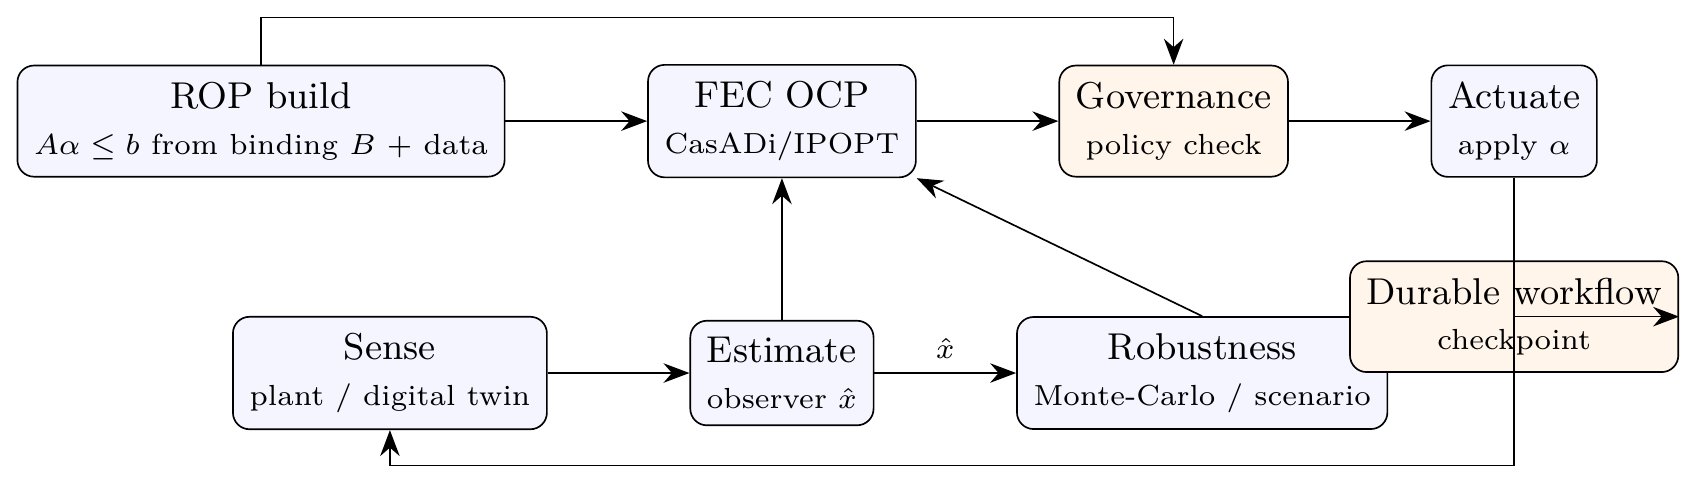
\includegraphics[width=16cm]{figures/ropfec_architecture.png}
\caption{\textbf{Figure 1.} Closed-loop \emph{reference} architecture implemented by \texttt{ropfec}. The ROP is
built once from binding stoichiometry and data and supplies hard constraints to the FEC
optimal-control problem and the governance check; the estimation, robustness, governance and
workflow blocks are reference implementations, not a production platform. The loop is
intended to supervise a staged-bioconversion process (deconstruction $\to$ kernel/handover
$\to$ recovery; the BOS pattern~\citep{paperA}), for which the ROP supplies the admissible
exponent geometry.}
\label{fig:arch}
\end{figure}

% =====================================================================
\section{Illustrative examples}\label{sec:examples}
% =====================================================================
All examples run on synthetic or published-model ground truth, with every number traceable
to a script in the repository.

\paragraph{(1) The ROP constraint matters for control (mechanism illustration).}
On a $3$-species, $4$-reaction glycolysis-like toy network (the Xiao running example) with a
six-facet binding-derived ROP, an exponent placed \emph{outside} the polytope gives a mean
trajectory error of $9.9\%$; the same exponent projected onto the ROP reduces it to $3.1\%$
(Figure~2), and the FEC solver, tracking a target
flux with a small regularizer toward the nominal exponent, returns an in-ROP solution within
$\sim2\%$ of the prescribed ground-truth exponent. This is a transcription/feasibility check,
not an identification result: pure flux tracking on this toy network is under-determined, so
the round-trip is driven mainly by the regularizer. On the same network the FEC solution
yields a final-state tracking cost no worse than the in-ROP FBA- and MM-derived exponent
policies ($1.01$ vs $1.28$ and $1.09$, a single deterministic evaluation). Because all three
policies are projected onto the same ROP, this compares policy heuristics under a shared
constraint and does not by itself attribute the cost gap to the binding geometry. A
scenario-robust variant bounds the worst case at near-nominal cost. These are internal sanity
checks on synthetic ground truth, not a performance benchmark. \emph{This is a mechanism illustration, not a benchmark}: the
ground truth is synthetic and the out-of-polytope baseline is, by construction, out of the
polytope, so the example demonstrates that respecting the binding constraint lowers the
synthetic-trajectory error, not empirical accuracy on biological data.

\begin{figure}[t]
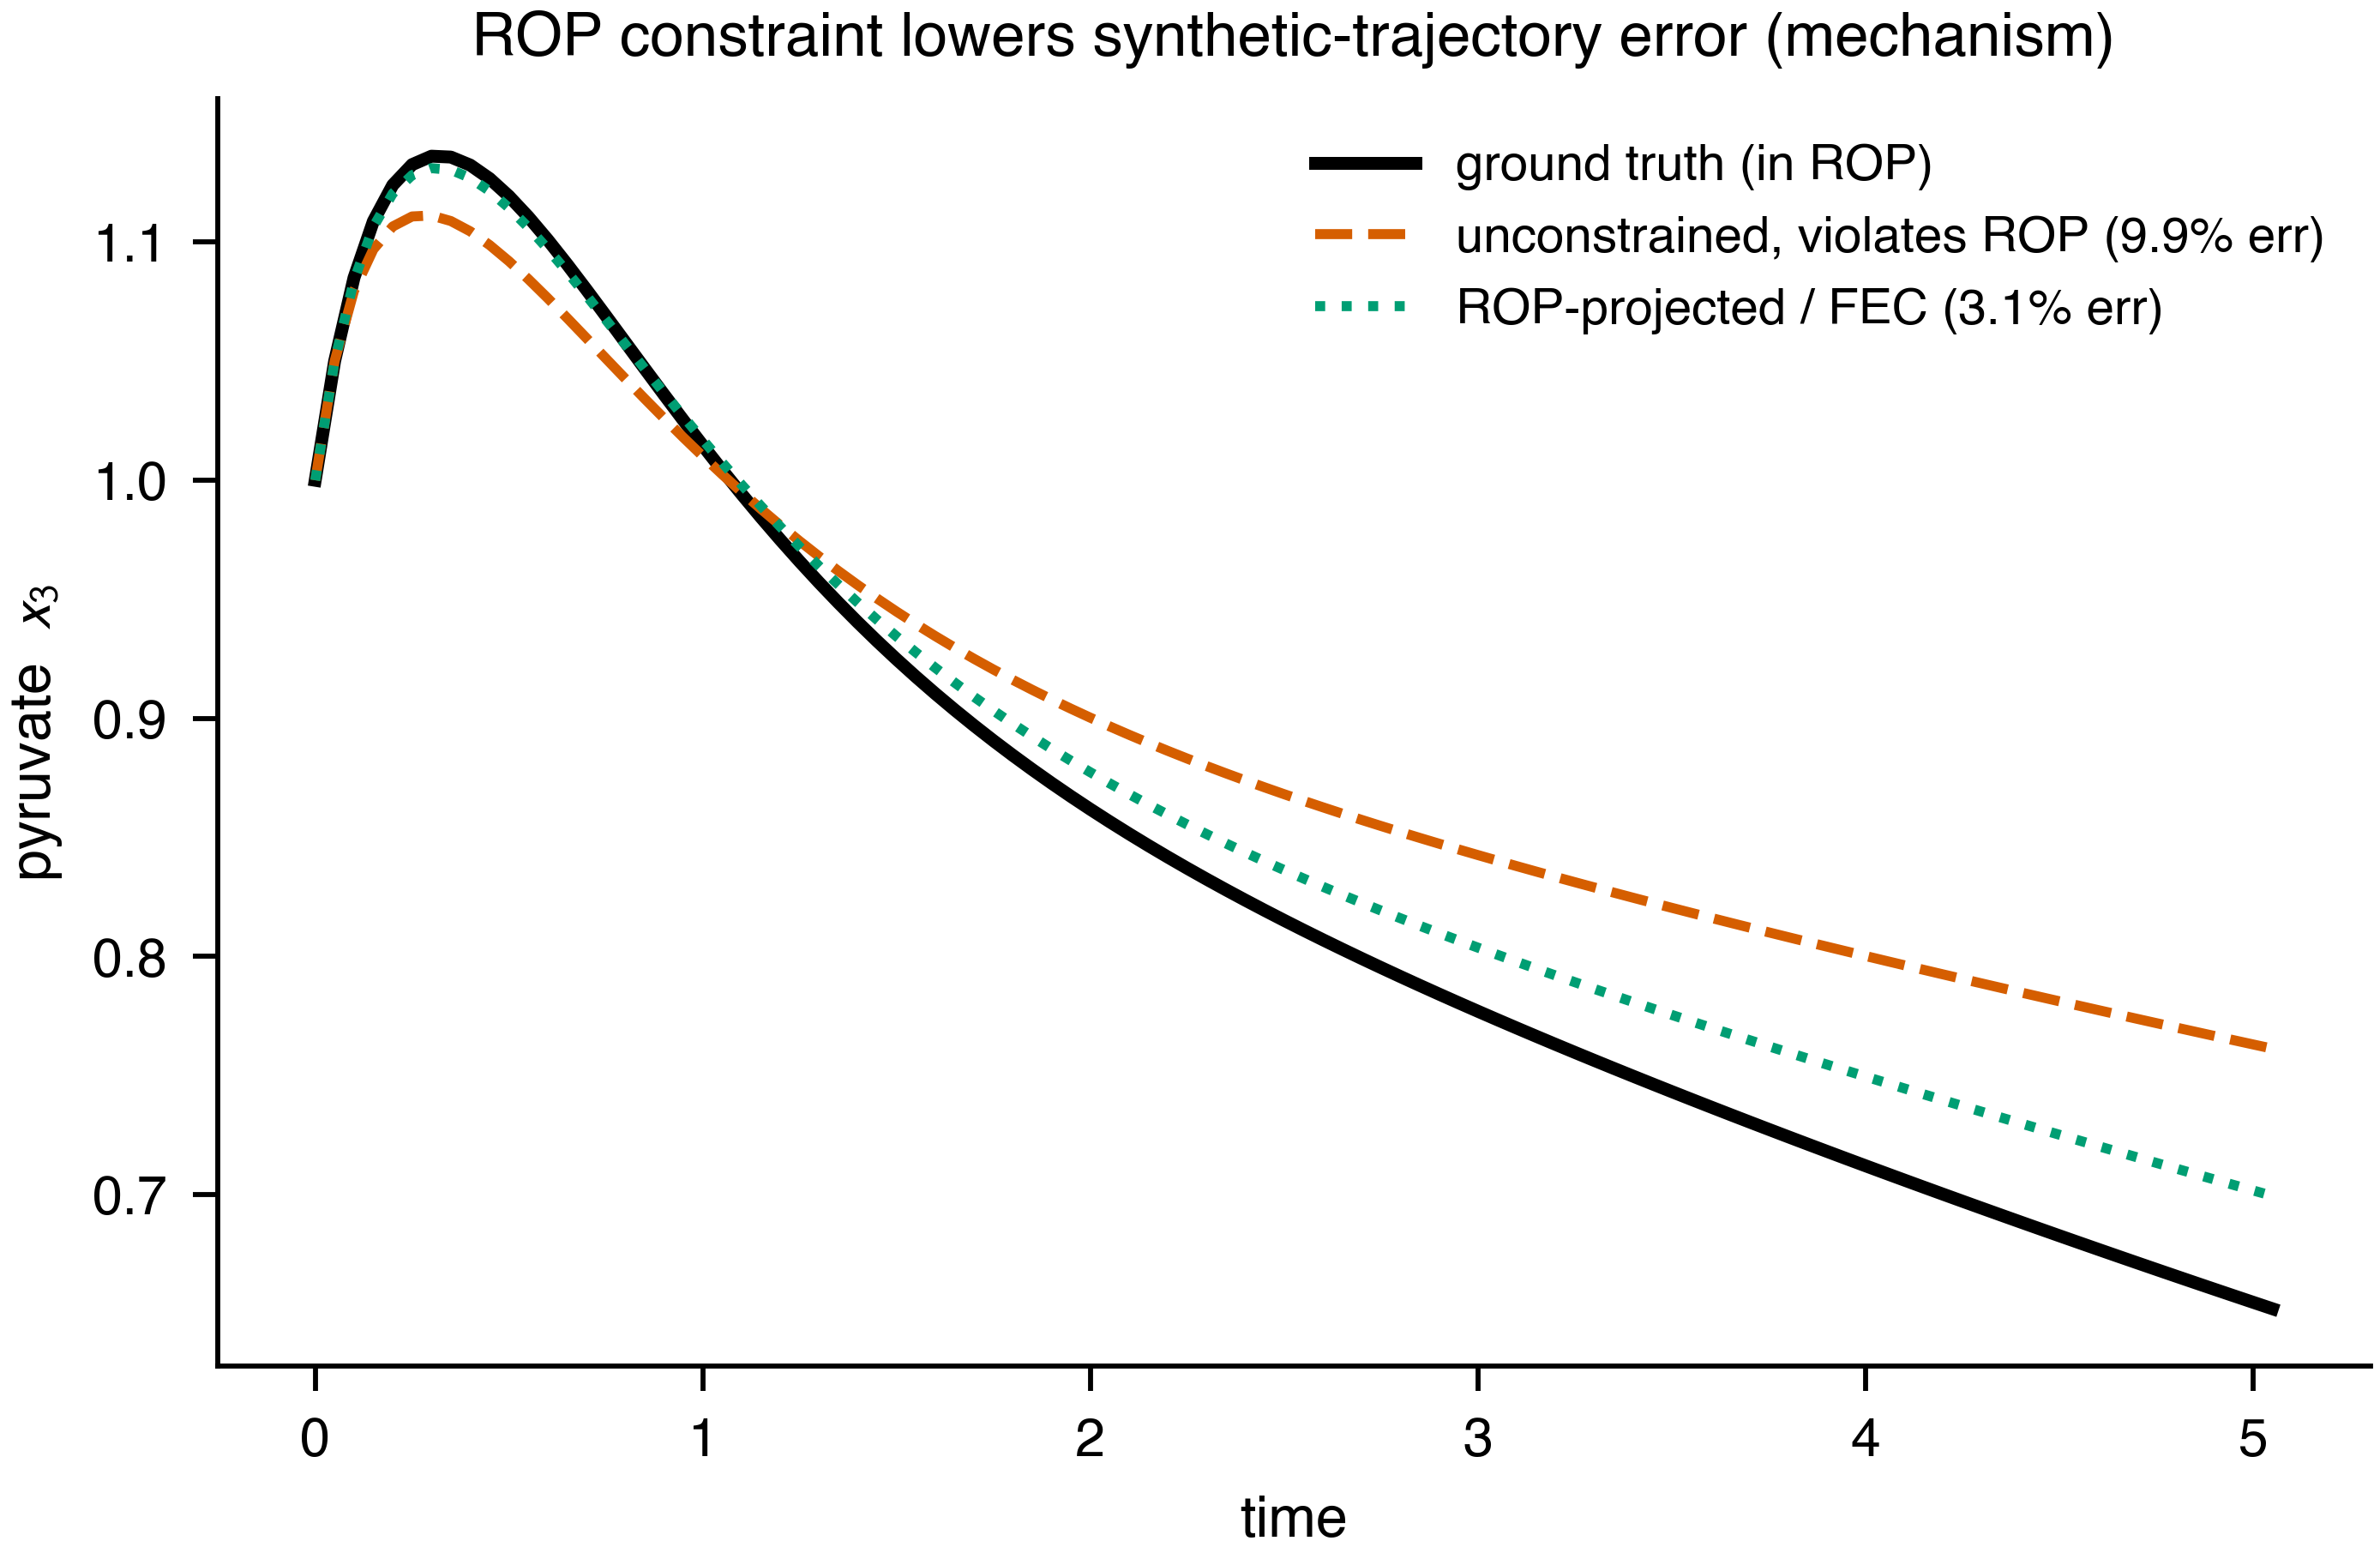
\includegraphics[width=12cm]{figures/toy_traj_comparison.png}
\caption{\textbf{Figure 2.} Mechanism illustration (in-silico): a state trajectory under the ground-truth
exponent, an unconstrained exponent that violates the ROP, and the ROP-projected/FEC
exponent. Respecting the binding-derived polytope lowers the synthetic-trajectory error (mean
$3.1\%$ vs $9.9\%$). Synthetic ground truth; not a biological benchmark.}
\label{fig:toy}
\end{figure}

\paragraph{(2) Validated oscillator testbeds.} The Sel'kov and Wolf--Heinrich
re-implementations reproduce the published qualitative behaviour (Figure~3):
Sel'kov settles onto a stable limit cycle inside its Hopf window and to a fixed point
outside it, and the Wolf--Heinrich single-cell core sustains glycolytic oscillations. Both
are asserted by tests and serve as reusable, citable testbeds for the FEC pipeline beyond
the toy network.

\begin{figure}[t]
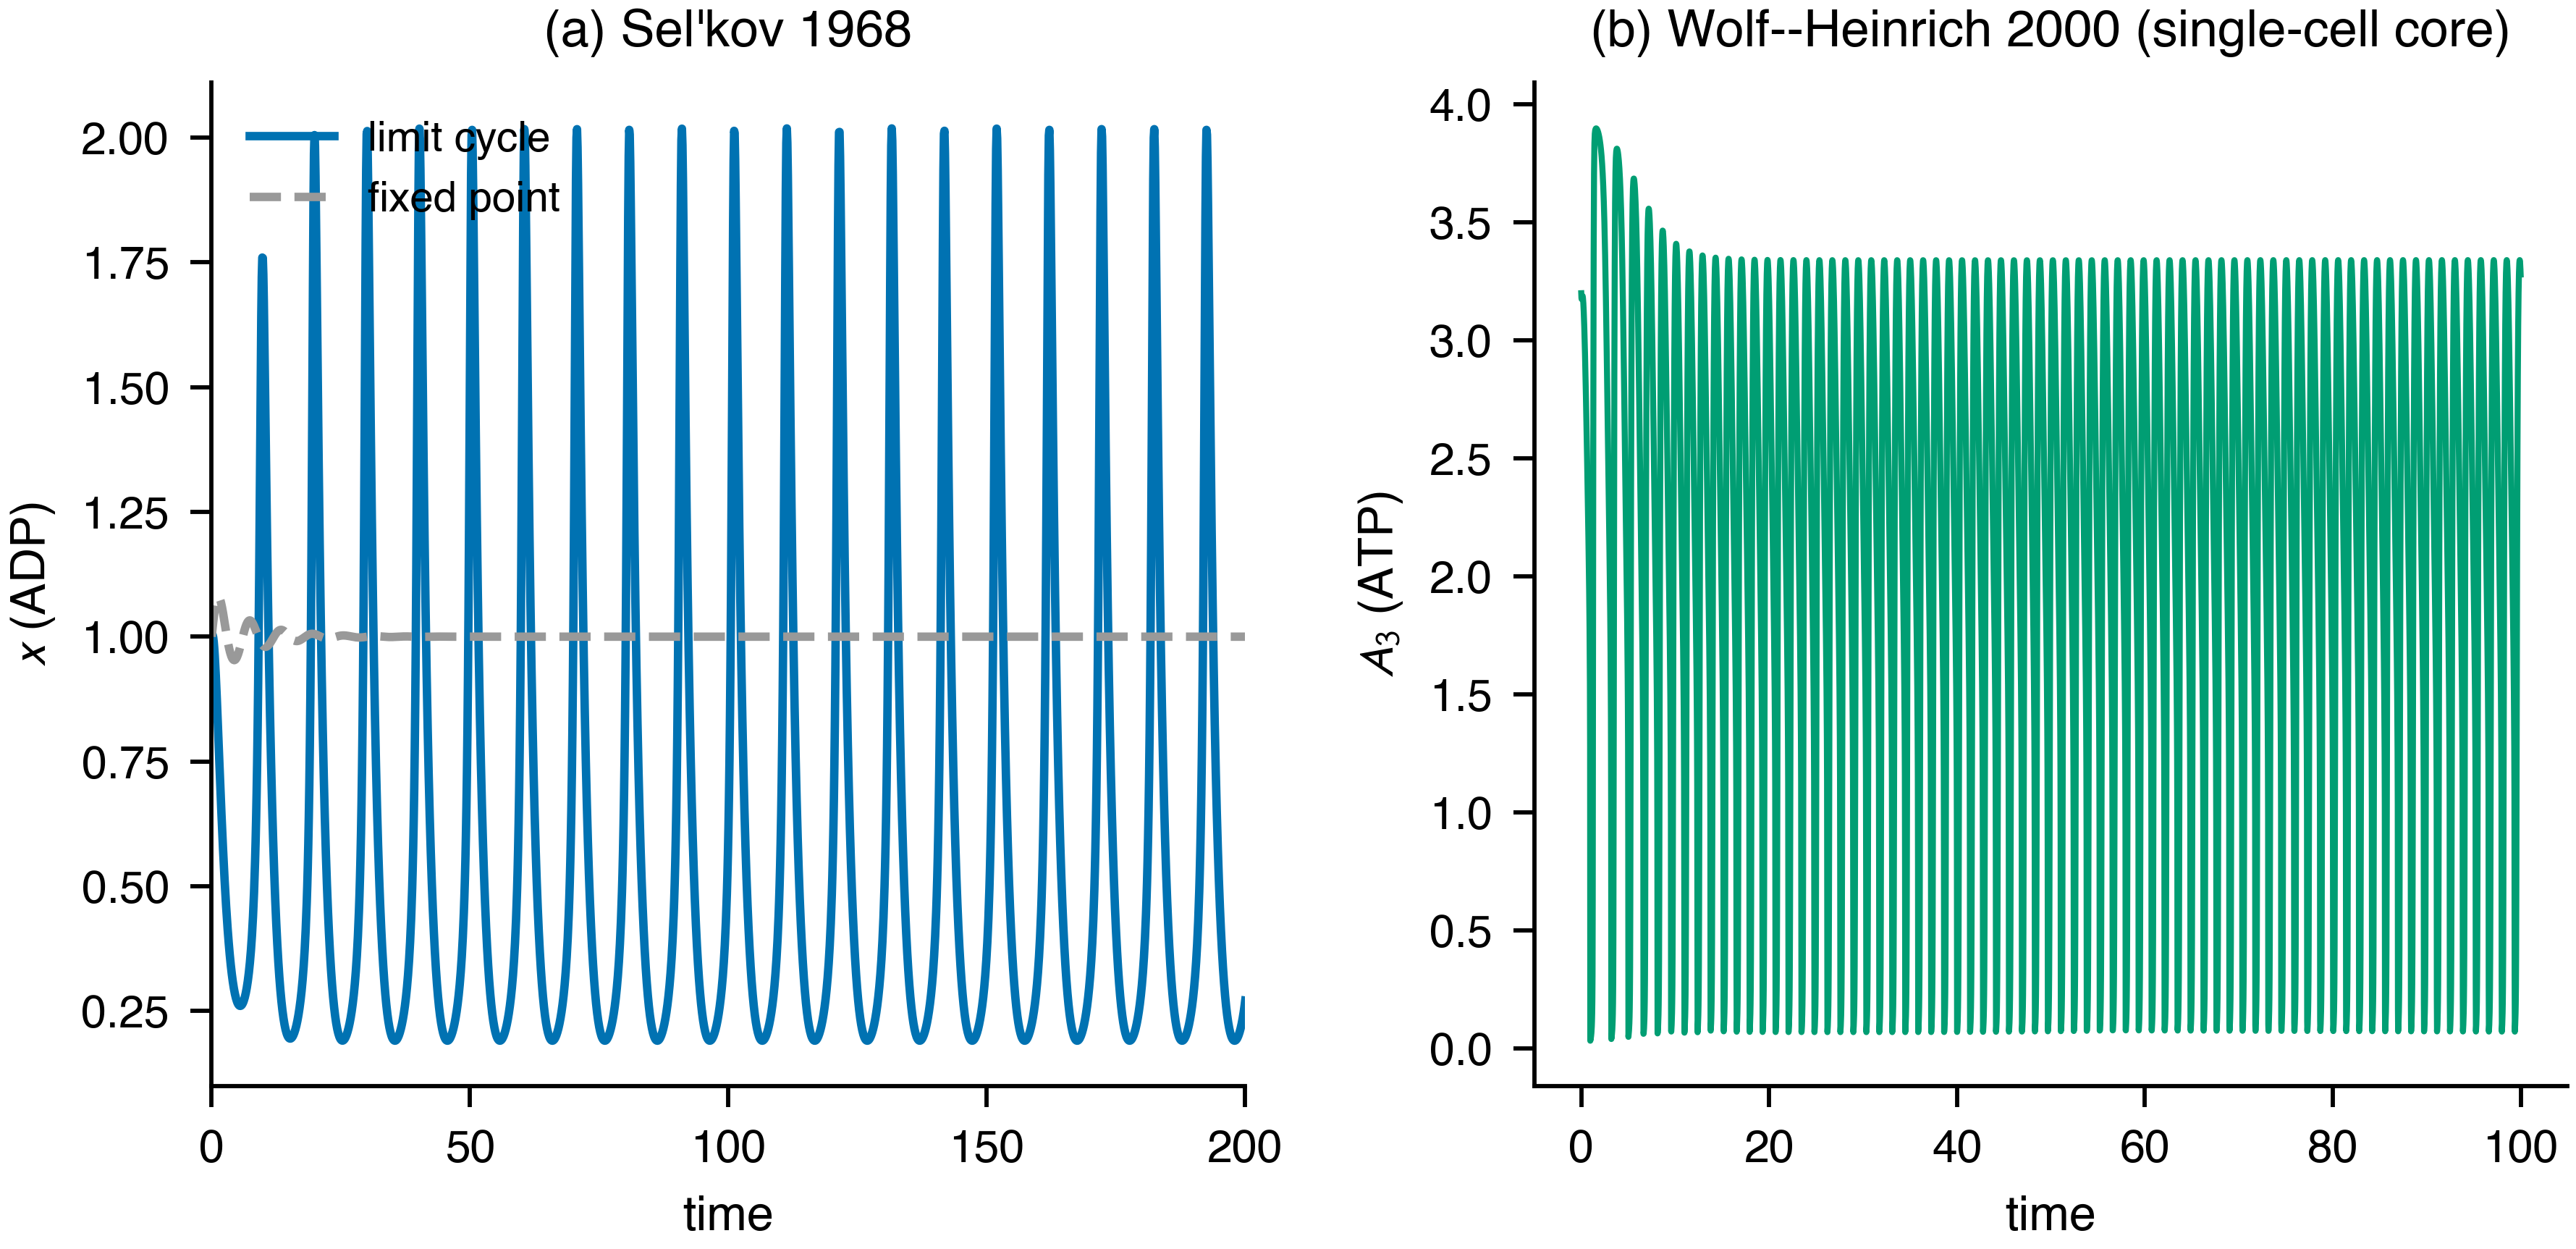
\includegraphics[width=16cm]{figures/case_studies_oscillations.png}
\caption{\textbf{Figure 3.} Validated re-implementations of two published glycolytic oscillators:
(a)~Sel'kov 1968 (limit cycle vs.\ damped fixed point); (b)~Wolf--Heinrich 2000 single-cell
core (sustained oscillation of an ATP-like cofactor). Tested against the published dynamics.}
\label{fig:osc}
\end{figure}

\paragraph{(3) Built-in falsification: structure does not aid identification.}
The central honest result, shipped as a test rather than buried as a caveat. A natural hope
is that the binding-derived ROP, used as a prior, tightens \emph{data-driven} estimation of
reaction orders. We test this against the right null. From noisy rate data we build the
bounded-error order set and compare three feasible sets: the data set alone, the data set
intersected with the ROP, and the data set intersected with a \emph{count-matched random}
facet set calibrated to still contain the true orders --- a control for ``more facets''
versus ``the right facets''~\citep{bental1998robust}. We measure total reaction-order
uncertainty in an informative regime and a data-poor regime (Figure~4).

The result is negative in substance. When data are informative the ROP is \emph{inactive}:
data, data$\cap$ROP, and data$\cap$random sets have identical order uncertainty
($\approx0.04$), so the data already constrain the orders more tightly than the ROP and its
facets never bind. When data are scarce both the ROP and the count-matched random null
tighten the set substantially below data-only ($2.72$), to $2.31$ and $2.34$ respectively
(60 seeds) --- a paired difference of only $\sim$1\% that is not statistically significant
(paired $t$-test $p\approx0.5$). The binding-derived structure therefore adds little to identification beyond a
generic constraint of equal size. The interpretation is clarifying rather than
discouraging, and it is the package's transferable thesis: the value of ROP/FEC is as a
structural \emph{control-admissibility set} --- the geometry the controller must respect
(example~1) --- \emph{not} as a statistical regulariser for \emph{identification}. Structure
constrains what the controller may do; it does not, by itself, tell you more about the plant
than the data already do. Running the full reference loop, every structural invariant holds:
the applied exponent is in the ROP at every step, the published polytope matches the
constructed one, governance violations are detected and counted, and the reference
multicellular policy rejects every over-capacity configuration in the test suite by its admission threshold.

\begin{figure}[t]
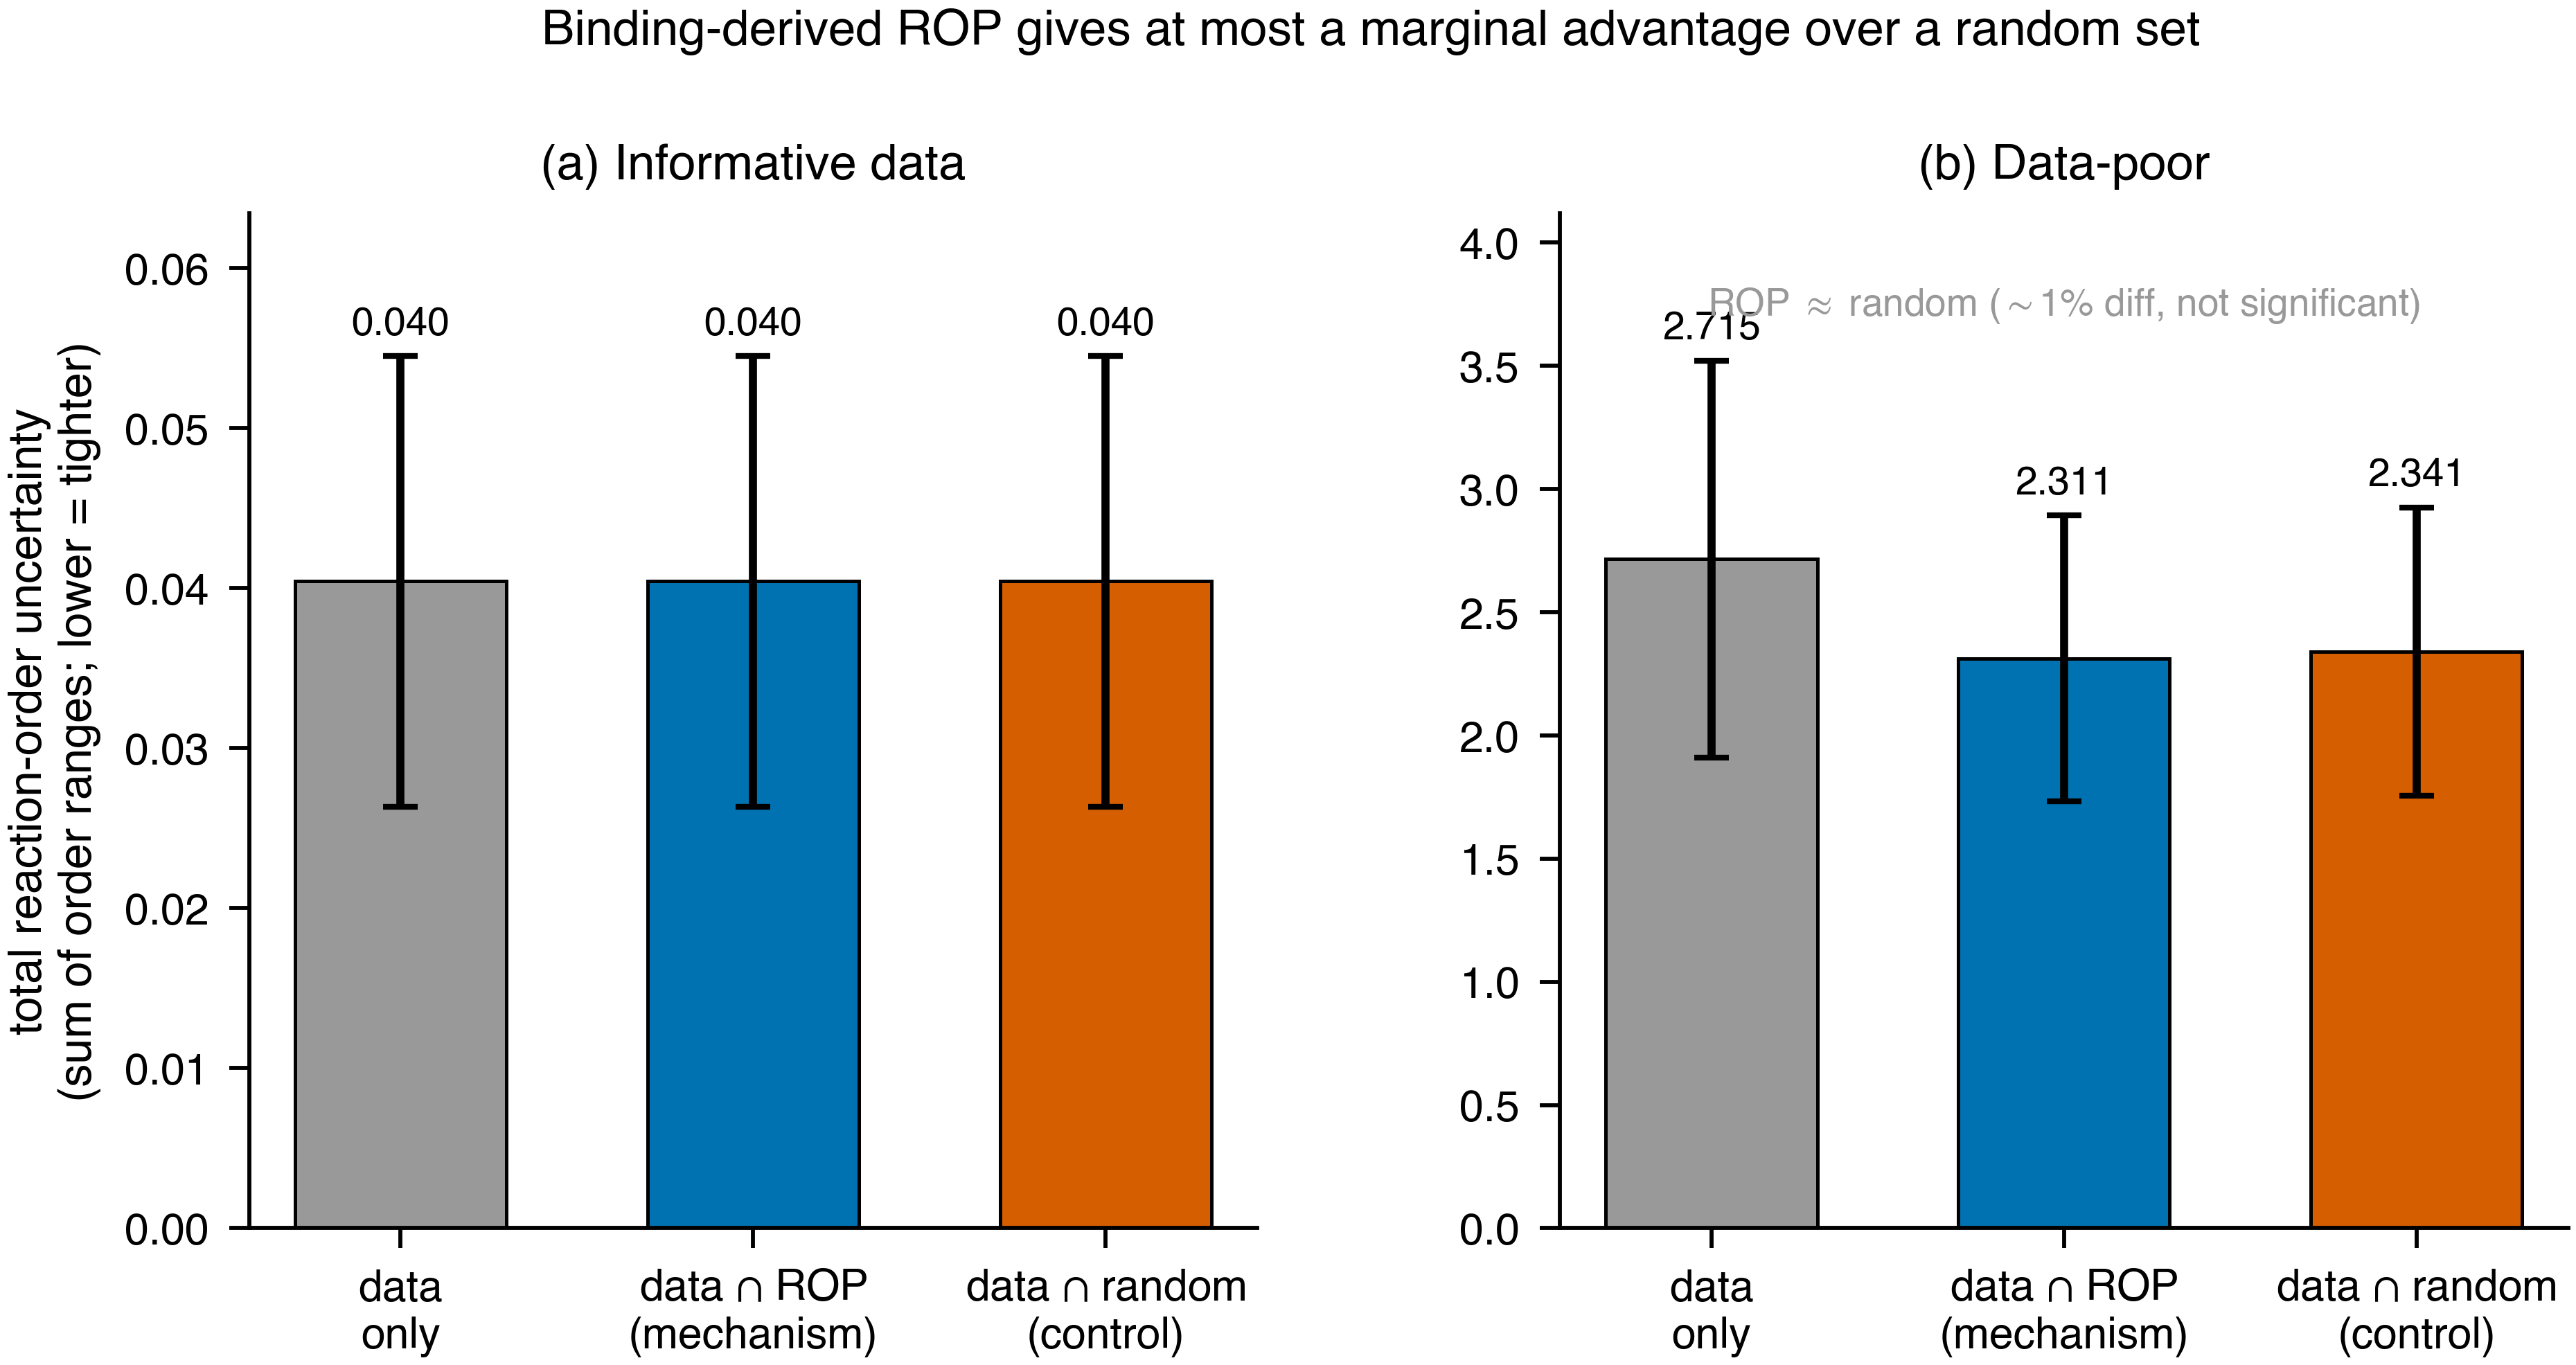
\includegraphics[width=\linewidth]{figures/order_uq_negative.png}
\caption{Built-in falsification (the package's central result; mean $\pm$ SD over 60 seeds).
Total reaction-order uncertainty for the data-only set, data$\cap$ROP, and data$\cap$random
(count-matched, truth-covering) sets, on independent scales for (a)~an informative and
(b)~a data-poor regime. The binding-derived ROP confers at most a marginal advantage over a
random set of equal size: when data are informative it is inactive (all three $\approx0.04$);
when data are scarce it tightens the set only $\sim$1\% more than the random null
(2.31 vs 2.34), a paired difference that is not statistically significant. Shipped as a re-runnable test.}
\label{fig:neg}
\end{figure}

% =====================================================================
\section{Impact}
% =====================================================================
\texttt{ropfec} provides an open, tested, citable implementation of a control framework
previously available mainly as theory and a model-predictive-control concept, with three concrete uses. \textbf{As infrastructure}, it is a reproducible
substrate for staged-bioconversion control research: the ROP/FEC core, the robust and
multicellular extensions, and the swappable reference loop let others prototype controllers
without re-deriving the geometry, and the two validated oscillators are ready-made testbeds.
The order-uncertainty module exposes importable primitives (\texttt{worst\_case\_range},
\texttt{bounding\_box}, \texttt{data\_halfspaces}, \texttt{estimate\_orders\_loglinear}), and the two
oscillator modules are imported directly by the 44-test suite.
\textbf{As pedagogy and grounding}, the explicit MCA-elasticity identity places FEC inside a
classical formalism that is familiar to the systems-biology and process-control communities,
making the control variable interpretable and unit-checkable. \textbf{As a methodological
caution}, the built-in falsification, with its count-matched random-facet null, is a
transferable template: it shows how to ask whether a \emph{structural} prior adds information
beyond a generic constraint of equal size, and reports the honest answer for this case
(it does not). By shipping self-skepticism as a test, the package makes the scope of the
framework auditable --- a responsible default for software that
operationalizes an attractive but unproven idea. Within the broader BOS software
ecosystem~\citep{paperA}, \texttt{ropfec} provides the candidate control-geometry layer; the empirical
resource-recovery results and the boundary-matched accounting are reported and reproduced
separately.

% =====================================================================
\section{Conclusions}
% =====================================================================
We presented \texttt{ropfec}, an open, tested, one-command-reproducible implementation of
reaction-order-polytope-constrained flux-exponent control for staged bioconversion. Beyond
the artifact, the package encodes two honest, re-runnable results: the clarifying identity
that FEC exponents are MCA elasticities, and a built-in falsification: against a count-matched random-facet null, the binding-derived
structure confers at most a marginal advantage for data-driven \emph{identification}; its
demonstrated role is instead as a \emph{control-admissibility set} (Example~1). The
work is offered as a reproducible reference and a map of where the framework adds
value, not as an overclaimed method; its scope is explicitly in-silico, with the wet-lab
system reported separately~\citep{paperA}.

% =====================================================================
\section*{Declarations}
% =====================================================================
\paragraph{Code and data availability.} The \texttt{ropfec} source, the 44 tests, and the
script that regenerates the data figures are released under the MIT license at
\url{https://github.com/exergyleizhou-ux/ropfec} (Table~1); a versioned snapshot
of the \texttt{v1.0.1} release will be archived with a DOI on Zenodo upon posting.
\paragraph{Use of generative AI.} Generative-AI tools assisted code and text drafting; the
author reviewed, verified, and is solely responsible for all content, including every
quantitative claim and citation, and reproduced all reported numbers from the released code.
\paragraph{Competing interests.} The author declares no competing interests.
\paragraph{Funding.} This research received no specific grant from funding agencies in the
public, commercial, or not-for-profit sectors.

\section*{Acknowledgements}
This work implements and builds upon the reaction order polytope and flux exponent control
framework of Fangzhou Xiao, Jing Shuang Li, and John C. Doyle.

\section*{References}
\end{document}
